\documentclass[12pt, twoside]{article}
\usepackage[letterpaper, margin=1in, headsep=0.5in]{geometry}
\usepackage[english]{babel}
\usepackage[utf8]{inputenc}
\usepackage{amsmath}
\usepackage{amsfonts}
\usepackage{amssymb}
\usepackage{tikz}
\usetikzlibrary{quotes, angles}
\usepackage{graphicx}
\usepackage{enumitem}
\usepackage{multicol}
\usepackage{hyperref}

\newif\ifmeta
\metatrue %print standards and topics tags

\title{IB Mathematics}
\author{Chris Huson}
\date{March 2022}

\usepackage{fancyhdr}
\pagestyle{fancy}
\fancyhf{}
\renewcommand{\headrulewidth}{0pt} % disable the underline of the header
\raggedbottom


\fancyhead[LE]{\thepage}
\fancyhead[RO]{\thepage \\ Name: \hspace{4cm} \,\\}
\fancyhead[LO]{BECA / IB Math 6 Geometry \\* 16 March 2022}

\begin{document}
\subsubsection*{6.3 The Law of Sines}
\begin{enumerate}
    \item Triangle $ABC$ has $\hat{A}=40^\circ$, $AB=7 \text{ cm}$, $BC=6 \text{ cm}$. Find the measure of $\hat{C}$:
    \begin{enumerate}
          \item Write down the law of sines, substituting appropriate values.\\[0.5in]
          \item Solve for the measure of angle $C$
    \end{enumerate}
    \begin{center}
    \begin{tikzpicture}[scale=0.6]
    \draw (0,0) node[anchor=north]{$A$}
      -- (12,0) node[anchor=north]{$C$}
      -- (6.75,6) node[anchor=south]{$B$}
      -- cycle;
      %(0,3) node[anchor=south]{$40^\circ$};
      %\draw [dashed] (1.5,0) -- (1.5,4.2);
    \end{tikzpicture}
    \end{center}

\newpage
\item Given a circle with radius of one, centered on the origin. An angle with measure $30^\circ$ is placed in standard position. Mark the point $A$, the intersection of the circle and angle ray, as an ordered pair.
    \begin{center}
    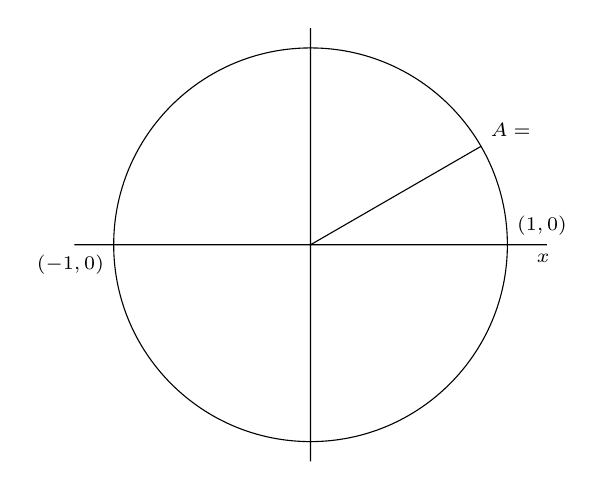
\begin{tikzpicture}[scale=2.5]
      \draw[font=\scriptsize]
        (-1.2, 0) -- (1.2, 0)
        (0, -1.1) -- (0, 1.1)
        (0, 0) -- (0.866, .5) node[above right] {$A=$}
        (0, 0) circle[radius=1]
        (-1, 0) node[below left] {$(-1,0)$}
        (1, 0) node[above right] {$(1,0)$}
        (1.1, 0) node[below right] {$x$}
        ;
    \end{tikzpicture}
    \end{center}
    \begin{enumerate}
          \item Write down the value of $\sin{30^\circ}$\\[0.25in]
          \item  Write down the value of $\cos{30^\circ}$\\[0.25in]
    \end{enumerate}
    
    
    

\end{enumerate}
\end{document}
